% https://tex.stackexchange.com/a/450851
\documentclass{beamer}
\usepackage{tikz}
\usetikzlibrary{matrix,overlay-beamer-styles}
\usetikzlibrary{positioning} %<- not important here
\begin{document}
 \begin{frame}[t]
 \frametitle{Matrix delimiters won't hide}

  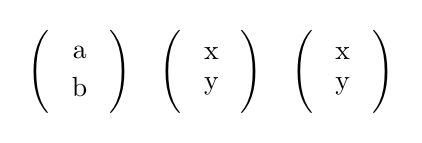
\begin{tikzpicture}[ampersand replacement=\&]
   \matrix [matrix of nodes,left delimiter=(,right delimiter=)] (m1)
     {
       a \\
       b \\
     };

   \tikzset{every delimiter/.append style={visible on=<2->}}
   \matrix [right=1cm of m1,visible on=<2->,matrix of nodes,
    left delimiter=(,right delimiter=)] (m2)
     {
       x \\
       y \\
     };
   \visible<3->{
      \matrix [right=1cm of m2,matrix of nodes,
       left delimiter=(,right delimiter=)] (m2)
        {
          x \\
          y \\
        };
   } 
  \end{tikzpicture}
 \end{frame}
\end{document}
